\documentclass{article}
\PassOptionsToPackage{numbers,compress,sort}{natbib}
\usepackage[preprint]{neurips_2025}
\usepackage[utf8]{inputenc}
\usepackage[T1]{fontenc}
\usepackage{hyperref,url,booktabs,amsfonts,amsmath,amssymb,microtype}
\usepackage{xcolor,graphicx,array,pifont,makecell}
\usepackage[font=small,labelfont=bf,skip=3pt]{caption}
\usepackage[shortlabels]{enumitem}
\usepackage{listings}
\lstset{basicstyle=\ttfamily\scriptsize,columns=fullflexible,keepspaces=true,frame=tb,
  framesep=3pt,showstringspaces=false,upquote=true,aboveskip=6pt,belowskip=4pt}
\graphicspath{{figures/}}
\hypersetup{pdftitle={High Attention, Low Contribution: A Fast-Weight Diagnosis of ViT Attention Maps},pdfauthor={Hongbo Huang},colorlinks=true,linkcolor=black,citecolor=blue!50!black,urlcolor=blue!50!black}
\newcommand{\up}{$^{\uparrow}$}
\newcommand{\dn}{$^{\downarrow}$}
\title{High Attention, Low Contribution:\\A Fast-Weight Diagnosis of ViT Attention Maps}
\author{Hongbo Huang \quad Student ID: 50026755\\\normalfont\texttt{\href{https://github.com/hhuang999/DSAA2012-vit-fastweight}{github.com/hhuang999/DSAA2012-vit-fastweight}}}
\begin{document}
\raggedbottom\clubpenalty=300\widowpenalty=300
\maketitle
\begin{abstract}
Deep-layer attention maps of vision transformers (ViTs) often highlight background patches rather than objects. Architectural remedies suppress these artifacts, yet why standard readouts mislead in frozen models remains unclear. We view each fixed-image head as a two-layer fast-weight network, with attention weights as hidden activations and projected values as output weights, to compare spatial priors, feature displacement, and low-norm outputs under matched controls. Although all three diagnostic premises hold in supervised DeiTs, only value weighting outperforms received attention and, on three of four alignment tests, its matched control, leaving an artifact-free DINO ViT-S unchanged; prior subtraction and relocation fail. Ablations reveal a spatially structured mismatch beyond extreme outliers, and experiments on DINOv2 and CLIP show trained registers substantially reduce spatial gains from value weighting, linking registers to post-hoc readouts. Finally, deletion and CLS interventions show that improved alignment and local contribution agreement do not reliably improve faithfulness.
\end{abstract}

\section{Introduction}
Attention maps are widely used to inspect vision transformers (ViTs)~\citep{dosovitskiy2021,touvron2021}, yet deep supervised layers often peak on background patches rather than objects (Fig.~\ref{fig:teaser}). Human-saliency agreement~\citep{linsley2019,fel2022} drops in final supervised layers while staying high in self-supervised DINO ViT-S~\citep{caron2021}. Existing remedies add register tokens~\citep{darcet2024,jiang2025}. Before altering models, we ask why frozen heads mislead and what their readouts reveal.

\begin{figure}[!h]\centering
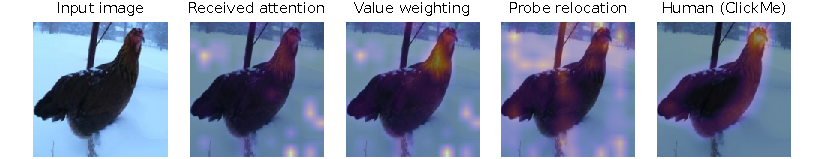
\includegraphics[width=0.68\linewidth]{teaser_maps}
\caption{Readouts of frozen DeiT-S over layers 9--12 on a ClickMe image (Sec.~\ref{sec:method}, App.~\ref{app:gallery}). Value weighting highlights the bird, whereas probe relocation disperses scores across the background.}\label{fig:teaser}
\end{figure}

To compare prior explanations together, we view each fixed-image head as a two-layer fast-weight network over queries~\citep{schmidhuber1992,schlag2021,wen2026mita}: keys act as first-layer weights, attention weights as hidden activations, and projected values as output weights. Standard maps show only activations. Following unit-level interpretability~\citep{bau2017}, background peaks can reflect an image-independent spatial bias, feature displacement across mixed tokens, or small output vectors despite high attention.

We make three contributions. First, we unify these explanations and test their readouts via paired diagnostics and matched controls (Sec.~\ref{sec:results}). Second, we show that attention--value decoupling extends beyond outliers and depends on spatial norm placement, linking registers to post-hoc readouts across model families (Sec.~\ref{sec:mech}). Third, we separate visual alignment, local contribution, and decision faithfulness via deletion and CLS interventions (Sec.~\ref{sec:boundary}).

\section{Related work}
\paragraph{Attention weights, token mixing, and value norms.} Fast-weight views of self-attention~\citep{schmidhuber1992,schlag2021,wen2026mita} separate how queries select source tokens from what they return. Norm analyses show attended tokens can carry small values~\citep{kobayashi2020}, motivating value-norm scaling~\citep{zhu2024} and multi-layer propagation~\citep{abnar2020,chefer2021generic,wu2024tokentm}. Separately, representation studies show deep tokens mix across patches rather than staying spatially anchored~\citep{brunner2020,raghu2021}. Prior work studies these factors in isolation or bundles them into multi-component heuristics, without matched controls separating spatial priors, mixing, and value norms.

\paragraph{High-input-norm tokens and attention sinks.} Supervised ViTs form background tokens with large block-input norms and small value outputs, which registers absorb during training or at test time~\citep{darcet2024,jiang2025}. Language-model massive activations and attention sinks likewise draw attention without proportional values~\citep{sun2024massive,xiao2024sinks,gu2025sink}. Yet existing work focuses on suppressing extreme outliers or modifying architectures, leaving open whether attention--value decoupling extends into non-outlier patches and how registers relate to post-hoc value weighting.

\paragraph{Evaluating attribution maps.} Agreement with human saliency reflects visual plausibility rather than decision faithfulness~\citep{jacovi2020,jain2019,wiegreffe2019}, and visual benchmarks face parameter-insensitivity~\citep{adebayo2018}, training-objective~\citep{walmer2023}, radial-bias, and occlusion confounds~\citep{petsiuk2018rise,bluecher2024}. Existing ViT readouts rarely separate visual alignment, local contribution, and input-level faithfulness under controls for these confounds, motivating our paired evaluation.

\section{Method}
\label{sec:method}
\paragraph{A head as a fast-weight network.} In our primary setup, a ViT maps a $224{\times}224$ image to $N=196$ patches ($14{\times}14$ grid) plus CLS. For head $h$ of dimension $d$, query $i$, and source $j$, let $z_j^h=W_O^h v_j^h$ denote the value vector projected by head $h$'s slice of the output matrix. Before residual addition, self-attention computes
\begin{equation}
 o_i=b_O+\sum_{h,j}a^h_{ij}z^h_j,\qquad
 a^h_{ij}=\mathrm{softmax}_j\big(q_i^{h\top}k_j^h/\sqrt{d}\big).
\label{eq:attn}
\end{equation}
Fixing the image makes $k_j^h/\sqrt{d}$ and $z_j^h$ first- and second-layer weights over queries $q_i^h$, with activations $a_{ij}^h$ (Fig.~\ref{fig:lens}). \emph{Received attention}, $s_j=\sum_{h,i}a_{ij}^h$, sums activations over heads and all 197 queries. \emph{Value weighting}, $c_j=\sum_{h,i}a_{ij}^h\|z_j^h\|_2$, sums source-$j$ contribution magnitudes, upper-bounding its aggregate net contribution across queries, $\sum_i\|\sum_h a_{ij}^h z_j^h\|_2$, by omitting cross-head cancellation.

\begin{figure}[!h]\centering
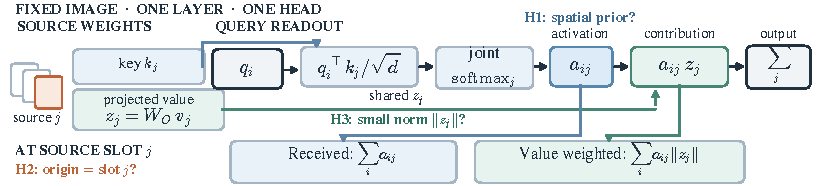
\includegraphics[width=0.54\linewidth]{fast_weight_lens}
\caption{Fast-weight view of one fixed-image head with keys $k_j$, activations $a_{ij}$, and outputs $z_j$.}\label{fig:lens}
\end{figure}

\paragraph{Unified diagnostics, modifications, and matched controls.} Each hypothesis pairs a diagnostic, modification, and matched control (App.~\ref{app:setup}). Under \emph{spatial prior} (H1), we measure variance in $s_j$ explained by a held-out mean map $\bar{s}_j$; \emph{mean-map subtraction} ($s_j-\bar{s}_j$) is controlled by a centred Gaussian of equal spread. Under \emph{feature displacement} (H2), a linear probe $P(p\mid x_j)$ predicts slot $p$ from token $x_j$; \emph{probe relocation} ($r_p=\sum_j s_j P(p\mid x_j)$) is controlled by matched-displacement Gaussian blur. Under \emph{low-norm output} (H3), we measure attention on $>3\times$ median input-norm outliers~\citep{darcet2024}; \emph{value weighting} is controlled by \emph{high-norm zeroing} ($s_j=0$ on outliers).

\paragraph{Evaluation protocol.} Primary tests aggregate layer-local readouts over layers 9--12 of frozen DeiT-S, DeiT-B~\citep{touvron2021}, and DINO ViT-S~\citep{caron2021}, fitting probes and mean maps on 4,000 ImageNet images. \emph{Same-ring enrichment} across 12,150 ImageNet-S masks~\citep{gao2023} measures excess foreground precision among top patches per equal-radius ring, scoring zero for radial maps. \emph{ClickMe alignment} (17,408 images) subtracts another image's saliency correlation from its own, removing fixed priors on average. The \emph{deletion score} (2,000 images) measures the area between least- and most-important-first top-1 retention curves after dropping patch tokens post-embedding~\citep{petsiuk2018rise,bluecher2024}. Verdicts require 95\% CIs excluding zero and $|\Delta|\ge 0.02$ ($0.05$ for deletion). Primary tests compare each modification with its matched control and their combination with received attention; other contrasts with received attention are descriptive (App.~\ref{app:setup}). Follow-ups use Oxford-IIIT Pet~\citep{parkhi2012pets}, DINOv2 ($518{\times}518$, $37{\times}37$ grid)~\citep{oquab2024dinov2}, and CLIP ViT-B/16~\citep{radford2021clip}.

\section{Experiments}
\label{sec:experiments}
\begin{figure}[!t]\centering
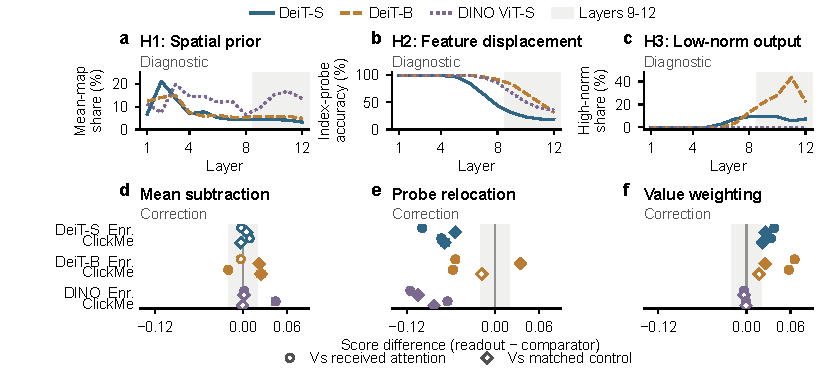
\includegraphics[width=0.70\linewidth]{diagnosis_correction_bridge}
\caption{Layer-wise diagnostics (a--c) and layers 9--12 readouts (d--f) versus received attention (circles) and matched controls (diamonds) with 95\% CIs; filled markers exceed $\pm0.02$ (grey bands; deletion in Table~\ref{tab:app-paired}).}\label{fig:diag}
\end{figure}

\subsection{Controlled evaluation of the three readout hypotheses}
\label{sec:results}
The diagnostic results support all three premises in deep supervised layers, showing that observational evidence alone cannot distinguish among the competing explanations (Fig.~\ref{fig:diag}a--c; Table~\ref{tab:app-diag}). Mean maps explain 3.3--16.7\% of spatial variance across models, while layer-12 position probes reach 18.1--35.7\% accuracy against 0.5\% chance. High-input-norm outliers attract up to 9.3\% of attention in DeiT-S and 43.5\% in DeiT-B versus 0\% in DINO ViT-S, with value norms only 0.29 and 0.23 times the median.

Controlled comparisons identify value weighting as the most effective alignment correction (Fig.~\ref{fig:diag}f; Table~\ref{tab:app-paired}). In DeiT-S and DeiT-B, it raises enrichment by 0.038--0.065 and ClickMe alignment by 0.033--0.058, closing 43--59\% of the gap to the gradient reference GAE~\citep{chefer2021generic}. Value weighting outperforms high-norm zeroing on three of four alignment tests, while DeiT-B ClickMe ($+0.017$) falls below 0.02. All DINO ViT-S metrics stay within 0.004 of received attention (negative control), and shuffling value norms within each head removes the gain, showing spatial arrangement matters (Table~\ref{tab:main}, App.~\ref{app:more}).

Neither alternative modification provides comparable gains. Mean-map subtraction mainly removes a radial bias already discounted by our metrics, matching centred Gaussian subtraction on DINO ClickMe (Fig.~\ref{fig:diag}d). Probe relocation lowers all three metrics by 0.054--0.161 (Fig.~\ref{fig:diag}e). Input-image patch masking on 64 pet crops shows why (App.~\ref{app:reloc}): background tokens assign 45--46\% of masking sensitivity to foreground patches, yet redistributing attention by this sensitivity still lowers alignment. Combining all three modifications improves only DeiT-B ClickMe alignment (App.~\ref{app:more}).

\subsection{Mechanism beyond extreme outliers and across pretraining regimes}
\label{sec:mech}
Zeroing $>3\times$ outliers recovers only 32--34\% of gains in DeiT-S and 61--70\% in DeiT-B, so we vary outlier and non-outlier weighting separately on 383 pet crops (Fig.~\ref{fig:mech}a; App.~\ref{app:more}). Weighting extreme outliers alone is less effective than removing them, whereas weighting remaining patches adds substantial gains. Non-outlier weighting plus outlier zeroing beats full value weighting, while within-ring shuffling removes the gain. Lowering the threshold to $1.5\times$ median flags 6--13\% of patches drawing 48--63\% of attention with small values and beats continuous weighting, revealing a graded tail.

\begin{figure}[!t]\centering
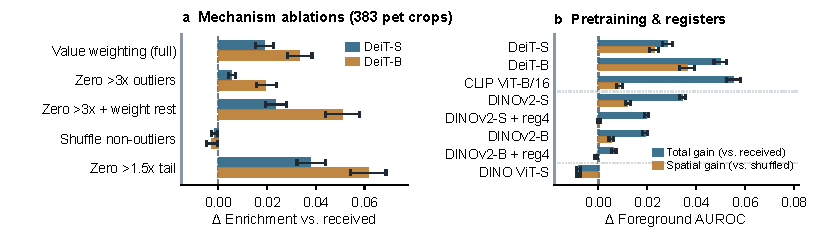
\includegraphics[width=0.90\linewidth]{mechanism_and_registers}
\caption{Exploratory ablations and cross-paradigm controls with 95\% CIs on 383--384 Oxford-IIIT Pet crops (App.~\ref{app:more}). (a) Enrichment shifts in DeiT-S and DeiT-B. (b) Total and spatial AUROC gains across regimes and registers.}\label{fig:mech}
\end{figure}

We next examine whether this mismatch appears under other pretraining regimes and whether trained registers reduce the need for value weighting (Fig.~\ref{fig:mech}b; App.~\ref{app:more}). Unregistered DINOv2 and CLIP ViT-B/16 form high-input-norm patches peaking at 37.4\% and 60.3\% of attention, where value weighting raises foreground AUROC by 0.019--0.055. Comparing with within-ring shuffling isolates spatial placement from head scaling. With four DINOv2 registers~\citep{darcet2024}, outliers vanish and baseline alignment rises; total gains fall by 42--67\% and spatial gains become negligible, linking value weighting to the spatial artifacts suppressed by registers.

\subsection{Visual alignment and decision faithfulness}
\label{sec:boundary}
Despite stronger visual alignment, post-embedding deletion gains remain modest (0.017 in DeiT-S, 0.029 in DeiT-B, below 0.05 and comparable to zeroing; Table~\ref{tab:app-paired}). A likely reason is query pooling, since standard maps aggregate all queries whereas only CLS feeds the classifier. On 128 pet crops, we hold block-12 attention fixed, remove each patch's CLS term $t_j=\sum_h a^h_{\mathrm{CLS},j}z_j^h$, and compare CLS readouts with margin changes and deletion (App.~\ref{app:explore}).

\begin{table}[!h]
\caption{Exploratory CLS-only minus all-query contrast for layer-12 value weighting with 95\% CIs (Sec.~\ref{sec:boundary}).}
\label{tab:cls}
\centering\footnotesize
\begin{tabular}{@{}lrrr@{}}
\toprule
Model & $\Delta$ Intervention $\rho$ & $\Delta$ Foreground AUROC & $\Delta$ Enrichment \\
\midrule
DeiT-S & +0.041 [0.026, 0.057] & $-$0.091 [$-$0.110, $-$0.074] & $-$0.033 [$-$0.043, $-$0.023] \\
DeiT-B & +0.082 [0.068, 0.096] & +0.024 [0.013, 0.036] & +0.005 [$-$0.005, 0.013] \\
\bottomrule
\end{tabular}

\end{table}

CLS value weighting improves internal-intervention correlation in both models (Table~\ref{tab:cls}), yet localisation and deletion diverge: foreground AUROC (Table~\ref{tab:cls}) and top-1 deletion fall in DeiT-S ($-0.031$) but rise in DeiT-B ($+0.026$), unaffected by cross-head cancellation (App.~\ref{app:explore}). These findings distinguish visual alignment, local intervention agreement, and decision faithfulness: better local agreement does not reliably improve localisation or input-level attribution.

\section{Discussion and conclusion}
Returning to our opening questions, the fast-weight framework explains why frozen maps mislead and closes three gaps. First, matched-control tests show that observing spatial priors, token mixing, or high-norm outliers does not prove their fixes work, isolating low projected values as the primary cause of background peaks. Second, moving beyond extreme-outlier studies, our ablations reveal a graded, spatially structured tail across non-outlier patches in supervised, self-supervised, and vision-language ViTs, while register-trained DINOv2 links this mismatch to architectural registers.

Answering what post-hoc readouts reveal, deletion and CLS tests resolve the conflation of plausibility and faithfulness. Output magnitudes recover alignment and CLS pooling tracks local branch contributions better, yet neither reliably improves faithfulness, so evaluations must match readouts to their target. Within our scope of frozen ViTs and layer-local readouts (App.~\ref{app:limitations}), dense prediction and cross-layer attribution remain open. Ultimately, attention weights describe how a head distributes weight across source tokens, not how strongly those tokens drive its output or final prediction.

\label{main:end}
\clearpage
{\footnotesize\setlength{\bibsep}{0.6pt}\bibliographystyle{plainnat}\bibliography{references}}
\clearpage\appendix
% =====================================================================================================
% Appendix: experimental details (A), additional results (B), tests of spatial relocation (C),
% example maps (D), details of placement and receiver tests (E), and key code (F).
% =====================================================================================================

\counterwithin{figure}{section}
\counterwithin{table}{section}
\captionsetup{skip=5pt}
\raggedbottom

\section{Experimental details}
\label{app:setup}

\paragraph{Models.}
All backbones are frozen ViTs operating on $224{\times}224$ inputs divided into $16{\times}16$ patches, loaded from \texttt{timm}~\citep{wightman2019}.
\emph{DeiT-S and DeiT-B}~\citep{touvron2021} use checkpoints \texttt{deit\_\allowbreak small\_patch16\_224.fb\_in1k} and \texttt{deit\_\allowbreak base\_patch16\_224.fb\_in1k} (resizing the short side to 248 followed by a $224{\times}224$ centre crop, a crop ratio of 0.9).
\emph{DINO ViT-S/16}~\citep{caron2021} uses checkpoint \texttt{vit\_\allowbreak small\_patch16\_224.dino} paired with its official linear classification head (resize to 256, centre crop to 224, crop ratio 0.875).
\emph{DeiT-S with a test-time register}~\citep{jiang2025} transfers the activations of eight selected feed-forward units in layers 4 and 5 onto a single appended register token, which is excluded from all spatial attribution maps alongside CLS. Those eight units were selected on 500 ImageNet-S images, where they reduce the per-layer count of high-norm patch tokens by 92.75\% while retaining 99.0\% of baseline predictions; on the remaining 11,919 images the reduction is 91.5\% and ImageNet accuracy remains at 79.8\%. Because the same search procedure did not identify comparably sparse units in DeiT-B (yielding only a 44.9\% reduction with 32 units), we evaluate the test-time register intervention on DeiT-S only.
\emph{Top-$k$ training} uses the released MiTA DeiT-S checkpoint~\citep{wen2026mita} (25 summary slots, $k=25$) under its native preprocessing (crop ratio 0.875). Because it differs from our DeiT-S backbone in both training objective and preprocessing, its entry in Table~\ref{tab:main} serves as descriptive context rather than a controlled comparison, and its deletion score is undefined because its summary slots pool fixed regions across the full patch grid. Both model-side comparisons are therefore restricted to size S.

\paragraph{Attention conventions.}
Letting $x$ denote the token representation after a block's first layer normalisation, the query, key and value projections retain the pretrained biases:
\[
q_i^h=W_Q^hx_i+b_Q^h,\quad k_j^h=W_K^hx_j+b_K^h,\quad v_j^h=W_V^hx_j+b_V^h.
\]
Eq.~\ref{eq:attn} includes the shared output-projection bias $b_O$ and describes the self-attention branch prior to residual addition, with dropout disabled at evaluation; $W_O^h$ denotes head $h$'s slice of the output projection matrix. Value weighting assigns each patch its per-head projected vector norm, leaving the shared bias $b_O$ unassigned. As illustrated in Fig.~\ref{fig:lens}, the fixed-image two-layer network interpretation couples hidden-unit activations through $\mathrm{softmax}_j$ rather than independent elementwise nonlinearities.

\paragraph{Datasets and evaluation splits.}
\emph{Execution sufficiency test}: 5,000 randomly sampled ImageNet validation images~\citep{deng2009}.
\emph{ImageNet-S}~\citep{gao2023}: all 12,419 validation images carrying semantic segmentation masks; enrichment is finite on 12,150 images (12,144 for DINO ViT-S under its 0.875 crop), while grids composed entirely of foreground receive zero enrichment. Restricting evaluation to crops containing both foreground and background patches alters the value-weighting enrichment contrast by less than 0.002 in every model, so reported verdicts follow the standard eligibility criterion. Deletion faithfulness is evaluated on a fixed random subset of 2,000 ImageNet-S images.
\emph{ClickMe}~\citep{linsley2019,fel2022}: the 17,408-image validation split distributed with Harmonization (17 \texttt{val-*.tfrecords} shards), whose shard names do not distinguish underlying ImageNet train/validation membership. Following Harmonization conventions, images are resized from $256{\times}256$ to $224{\times}224$ without cropping, and human saliency maps are resized to $64{\times}64$, smoothed with a $10{\times}10$ Gaussian kernel ($\sigma=10$), and bilinearly upsampled to $224{\times}224$.
\emph{Held-out calibration set}: 4,000 ImageNet validation images excluded from all map-quality and execution evaluations; 2,000 images are used to fit position probes and 2,000 are reserved for computing held-out mean maps, probe test accuracies and Gaussian blur widths. A near-duplicate check matched 2 of 4,002 candidate validation images to ClickMe records, which cannot rule out broader overlap between ClickMe images and ViT pretraining sets and therefore bounds generalisation claims.

\paragraph{Per-layer diagnostics.}
Each diagnostic corresponds directly to hypotheses H1--H3 in Sec.~\ref{sec:method} and is evaluated per layer.
\emph{Specificity (H1: spatial prior)}: letting $\bar s$ be the mean received-attention map on the 2,000 held-out calibration images and $\operatorname{Var}_j$ be the variance across the 196 patches of image $x$, the variance share explained by the dataset mean is $1-\sum_x\operatorname{Var}_j(s-\bar s)\,/\sum_x\operatorname{Var}_j(s)$, summed over ImageNet-S images $x$.
\emph{Location (H2: feature displacement)}: the top-1 classification accuracy of the 196-way linear position probe evaluated across all 196 patch tokens of the 2,000 held-out test images.
\emph{Output magnitude (H3: low-norm output)}: the fraction of ImageNet-S received attention falling on high-norm patches. The high-norm criterion (block-input norm exceeding three times the per-image median) is an operational definition fixed before running the main experiments without threshold tuning; value weighting itself requires no threshold.

\paragraph{Readout modifications and matched controls.}
Readout scores are computed per layer and summed across layers 9--12 without per-layer rescaling (except for calibrating the Gaussian control below). All three baseline models sum over all 197 queries (including CLS) and evaluate scores strictly over the 196 patch tokens.
\emph{Mean-map subtraction} computes $\sum_\ell(s_\ell-\bar s_\ell)$ using the 2,000 calibration images and retains negative values when ranking patches without clipping. Writing $S=\sum_\ell s_\ell$ and $\bar S=\sum_\ell\bar s_\ell$, its matched control subtracts a scaled centred isotropic Gaussian, $S-G\,\operatorname{sd}_j(\bar S)/\operatorname{sd}_j(G)$, where $G$ has width $\sigma=3.5$ patches, matching the spread of the summed mean map.
\emph{Probe relocation} computes \mbox{$r_p=\sum_j s_jP_\ell(p\mid x_j)$}, conserving total map mass. For each model and layer, a 196-way linear classifier is trained on layer-normalised tokens after the first LayerNorm (standardised using training-set mean and standard deviation floored at $10^{-6}$) via cross-entropy with Adam (learning rate 0.01, 30 epochs, token minibatches of 4,096, seed 0) on the 2,000 probe-training images. Its matched Gaussian blur control applies a row-normalised kernel $K_{jp}\propto\exp(-\lVert p-j\rVert^2/(2\sigma_\ell^2))$ whose width $\sigma_\ell\in[0.7, 2.9]$ patches matches the probe's mean squared displacement on the 2,000 calibration images,
\[
D_\ell=\frac{1}{2000N}\sum_{x,j,p}P_\ell(p\mid x_j)\lVert p-j\rVert^2,
\]
averaged uniformly across source patch indices. ClickMe evaluates the same crop-trained probes and blur widths on uncropped resized images, introducing a potential geometric mismatch.
\emph{Value weighting} computes $c_j=\sum_{h,i}a_{ij}^h\lVert W_O^hv_j^h\rVert_2$, a sum of per-head norm-weighted terms related to \citet{kobayashi2020}; taking each head's Euclidean norm prior to summation omits cancellation across heads, and residual addition, layer normalisation and downstream blocks lie outside this single-layer score. Its matched control zeros received attention on high-norm patches whose residual-stream block-input norm \emph{before} the first LayerNorm exceeds three times the per-image midpoint median norm; value weighting itself imposes no threshold.
\emph{Combined modification}: applying value weighting, followed by probe relocation, followed by subtracting the held-out mean of the resulting relocated map per layer prior to summation across layers 9--12.

\paragraph{Evaluation metrics and statistical inference.}
\emph{Same-ring object enrichment}: a patch is valid if it contains at least one non-ignored pixel and is labelled foreground if at least half of its non-ignored pixels fall inside the class mask. Selecting as many top-scoring valid patches as there are foreground patches, we compute within each ring of equal centre distance the foreground fraction among selected patches minus that among all valid patches in that ring, averaging across rings weighted by selected patch count. Invalid patches are excluded from selection and baselines, ties are broken with fixed seeded noise, and a purely radial map yields zero enrichment in expectation.
\emph{Image-specific ClickMe alignment}: each map is bilinearly upsampled to $224{\times}224$ and correlated (pixel Spearman $\rho$) with its matching human saliency map; to remove fixed spatial priors on average, we subtract the correlation with the preceding image's human map within each batch (\texttt{roll(1)}, batch size 64). While this permutation yields zero expected difference for any image-independent map, individual-image differences vary and the control does not enforce strict invariance when a fixed prior mixes with image-dependent signal.
\emph{Deletion score}: patches are ranked once from the unmodified map, and at removal budgets $0,1,2,4,8,16,32,64,98,147$ we record binary preservation of the unmodified top-1 class prediction when dropping patch tokens after positional embedding (keeping CLS and any register token). Following the Symmetric Relevance Gain (SRG) formulation~\citep{bluecher2024}, we compute the least-important-first minus most-important-first (LIF--MIF) trapezoidal area integral over removed patch fraction $b/196$ from 0 to $147/196$, replacing continuous class probability with binary top-1 retention.
\emph{Metric calibration controls}: a random uniform map, a centred Gaussian and the dataset-mean map all score within 0.004 of zero on enrichment and ClickMe alignment (with zero mean up to numerical precision on ClickMe for the two image-independent maps). On deletion, however, the centred Gaussian alone achieves 0.110, 0.099 and 0.140 (DeiT-S, DeiT-B, DINO ViT-S), underscoring why every readout edit must be evaluated against a matched control.
\emph{Statistical testing}: using one summary value per image, uncertainty is estimated via paired image-bootstrap resampling (1,000 draws, seed 0, 95\% percentile intervals, unadjusted for multiplicity). A paired difference is classified as \emph{higher} (\textit{h}) or \emph{lower} (\textit{l}) only if its 95\% CI excludes zero and its absolute mean meets the practical-significance threshold of 0.02 for alignment metrics (0.05 for deletion), and \emph{comparable} (\textit{c}) otherwise (which also covers imprecise differences). Bootstrap resampling conditions on fixed checkpoints, probes and ClickMe batch pairings. To verify robustness against within-batch ClickMe dependence (since each control pairs adjacent images inside 64-image batches), a sensitivity check resampling the 272 original batches intact yields 95\% CIs of [0.021, 0.023] in DeiT-S and [0.016, 0.018] in DeiT-B for value weighting versus high-norm zeroing.

\paragraph{Gradient attribution reference.}
The gradient-based attribution baseline (GAE)~\citep{chefer2021generic} targets the unmodified top-1 logit across all 12 layers. Initialising $R=I$, each layer updates $R\leftarrow R+\operatorname{mean}_h[(\nabla_{A^h}f_c\odot A^h)_+]R$ before extracting the final CLS-to-patch row. Because GAE is class-specific and spans all 12 blocks whereas our evaluated readouts are class-agnostic and sum layers 9--12, GAE scores serve as upper-reference context rather than a single-component ablation.

\paragraph{Pre-registered predictions.}
Table~\ref{tab:app-registered} summarises all hypotheses fixed prior to the main evaluation runs (following 32--64-image smoke checks), retaining the archived pre-registration labels P1--P7 to preserve exact traceability to the original protocol record; supplementary mechanism analyses were specified post hoc. P1 and P2 replicate prior execution and per-layer diagnostic profiles. Under P7, the pre-specified primary comparisons are the combined three-edit readout against received attention (P3) and each single edit against its matched control (no predicted direction for the single-edit controls); P4a and P4b state negative-control invariance expectations, while other individual comparisons against received attention are descriptive. P3 predicted improvements across all four supervised alignment comparisons (DeiT-S and DeiT-B on enrichment and ClickMe), under a decision rule classifying four higher outcomes as ``holds'', one to three as ``partly holds'' and zero as ``does not hold''; observing one higher, one comparable and two lower outcomes thus formally falls under ``partly holds'' and refutes a general improvement.

\begin{table}[!htbp]
\caption{Archived pre-registered predictions (P1--P7) and observed verdicts on the centre-controlled alignment metrics (same-ring enrichment and ClickMe alignment) unless otherwise noted.}
\label{tab:app-registered}
\centering\footnotesize
\setlength{\tabcolsep}{4pt}
\begin{tabular}{@{}l>{\raggedright\arraybackslash}p{3.45in}>{\raggedright\arraybackslash}p{1.45in}@{}}
\toprule
ID & Pre-registered prediction & Observed outcome\\
\midrule
P4a & Value weighting is comparable to received attention in DINO ViT-S on all three metrics & holds (3 of 3 comparisons)\\
P4b & Relocation at layers 1--4 is comparable to received attention on centre-controlled metrics in all models & holds (6 of 6 comparisons)\\
P3 & Combining all three modifications exceeds received attention on centre-controlled metrics in DeiT-S and DeiT-B & partly holds (1 higher: DeiT-B ClickMe; 1 comparable; 2 lower)\\
P6 & Neither model-side change exceeds DeiT-S received attention on centre-controlled metrics & holds (4 of 4 comparisons)\\
\midrule
P1 & Execution agreement increases with $k$ and exceeds size-matched random key sets at every $k$ & holds across all models\\
P2 & Probe accuracy declines with depth; high-norm attention share peaks in layers 6--12 of supervised ViTs and stays below 1\% in every layer of DINO ViT-S & holds across all models\\
\bottomrule
\end{tabular}
\end{table}

\paragraph{Model-side baselines: test-time register and MiTA.}
Both model-side baselines alter the forward pass rather than how a frozen head is read. The test-time register transfers selected feed-forward activations to an auxiliary token to mitigate high-norm outliers, whereas the released MiTA checkpoint alters both attention routing and training dynamics; neither modifies the fixed-image two-layer representation of our frozen baseline. Under P6, neither model-side alternative exceeded the 0.02 alignment threshold over DeiT-S received attention across all four comparisons, though MiTA's distinct training regime and crop preprocessing limit direct comparison.

\paragraph{Compute and code availability.}
Original GPU sweeps required approximately 19 NVIDIA L4 GPU hours. Our \href{https://github.com/hhuang999/vit-fastweight-lens}{code repository} maps every figure and table to its generating scripts and provides separate workflows to rebuild displays from preserved outputs or rerun full inference.

% =====================================================================================================
\section{Additional results}
\label{app:more}

We first document absolute evaluation scores and execution sufficiency sweeps, followed by the full paired contrasts plotted in Fig.~\ref{fig:diag} and post-hoc mechanistic checks on value weighting and parameter sensitivity.
\suppressfloats[t]

\begin{center}\begin{minipage}{\linewidth}
\captionof{table}{Complete evaluation scores for layers 9--12 unless stated otherwise. Arrows indicate higher or lower scores relative to received attention (DeiT-S for model-side rows); diamonds indicate higher scores than the matched control; bold marks higher than both comparators; untagged tested entries are comparable. GAE uses gradients over all 12 layers; dashes denote undefined or untested comparisons.}
\label{tab:main}
\centering\footnotesize\setlength{\tabcolsep}{2.6pt}
% Generated from results/table1_long.csv, correct_tests.csv and variants.csv.
\begin{tabular}{@{}l@{\hspace{4pt}}rrr@{\hspace{7pt}}rrr@{\hspace{7pt}}rrr@{}}
\toprule
 & \multicolumn{3}{c}{DeiT-S} & \multicolumn{3}{c}{DeiT-B} & \multicolumn{3}{c}{DINO ViT-S}\\
\cmidrule(r{6pt}){2-4}\cmidrule(r{6pt}){5-7}\cmidrule{8-10}
Readout & Enr. & Click. & Del. & Enr. & Click. & Del. & Enr. & Click. & Del.\\
\midrule
Received attention & 0.140 & 0.157 & 0.236 & 0.080 & 0.107 & 0.169 & 0.199 & 0.208 & 0.285 \\
Value weighting & \textbf{0.178}$^{\uparrow\diamond}$ & \textbf{0.190}$^{\uparrow\diamond}$ & 0.253 & \textbf{0.146}$^{\uparrow\diamond}$ & 0.165$^{\uparrow}$ & 0.198 & 0.196 & 0.207 & 0.285 \\
\quad high-norm zeroing (control) & 0.152 & 0.168 & 0.241 & 0.121$^{\uparrow}$ & 0.148$^{\uparrow}$ & 0.186 & 0.199 & 0.208 & 0.285 \\
Mean-map subtraction & 0.138 & 0.165 & 0.208 & 0.077$^{\diamond}$ & 0.087$^{\downarrow\diamond}$ & 0.144$^{\diamond}$ & 0.201 & 0.252$^{\uparrow}$ & 0.233$^{\downarrow}$ \\
\quad centred-Gaussian subtraction (control) & 0.133 & 0.168 & 0.167$^{\downarrow}$ & 0.056$^{\downarrow}$ & 0.062$^{\downarrow}$ & 0.024$^{\downarrow}$ & 0.200 & 0.253$^{\uparrow}$ & 0.232$^{\downarrow}$ \\
Probe relocation & 0.041$^{\downarrow}$ & 0.084$^{\downarrow}$ & 0.076$^{\downarrow}$ & 0.027$^{\downarrow\diamond}$ & 0.050$^{\downarrow}$ & 0.051$^{\downarrow}$ & 0.084$^{\downarrow}$ & 0.143$^{\downarrow}$ & 0.141$^{\downarrow}$ \\
\quad matched-displacement blur (control) & 0.095$^{\downarrow}$ & 0.152 & 0.181$^{\downarrow}$ & $-$0.008$^{\downarrow}$ & 0.068$^{\downarrow}$ & 0.097$^{\downarrow}$ & 0.189 & 0.226 & 0.287 \\
All three corrections & 0.059$^{\downarrow}$ & 0.123$^{\downarrow}$ & 0.076$^{\downarrow}$ & 0.079 & 0.137$^{\uparrow}$ & 0.085$^{\downarrow}$ & 0.088$^{\downarrow}$ & 0.177$^{\downarrow}$ & 0.090$^{\downarrow}$ \\
\midrule
+ test-time register & 0.152 & 0.169 & 0.236 & -- & -- & -- & -- & -- & -- \\
Top-$k$ training (MiTA) & 0.100\dn & 0.115\dn & -- & -- & -- & -- & -- & -- & -- \\
GAE (reference) & 0.204 & 0.234 & 0.345 & 0.196 & 0.213 & 0.308 & 0.221 & 0.234 & 0.418 \\
\bottomrule
\end{tabular}

\end{minipage}\end{center}
\begin{samepage}\paragraph{Execution sufficiency test.}
To test whether top-$k$ attended keys account for unmodified predictions, the $14{\times}14$ patch grid is partitioned into 16 overlapping spatial regions. In every layer and head, each region's mean query selects its top-$k$ keys (CLS retains its own key set), and in a subsequent forward pass every query is restricted to attend only to its region's selected key subset across all 12 layers simultaneously. Top-$k$ key sets consistently outperform size-matched random key sets at every tested $k$ (4--128) across all models, with top-1 agreement rising monotonically with $k$ (Fig.~\ref{fig:app-ksweep}).

\par\end{samepage}
\begin{center}\begin{minipage}{3.6in}
\centering
\includegraphics[width=3.25in]{execution_k_sweep}
\captionof{figure}{Top-1 agreement with unmodified predictions on 5,000 ImageNet validation images when restricting keys to region-selected top-$k$ subsets (solid), random subsets (dashed) or removing self-attention (dotted). All 95\% confidence intervals are within $\pm1.5$ percentage points; dotted curves use crop ratio 0.875 across models whereas solid and dashed curves use each checkpoint's standard preprocessing.}
\label{fig:app-ksweep}
\end{minipage}\end{center}

\paragraph{Per-layer diagnostics.}
Distance from the grid centre explains 82--98\% of held-out mean-map variance across layers 9--12. In a preliminary analysis across 11,919 ImageNet-S images (uniform 0.875 crop ratio; main DeiT runs use 0.9), we quantified raw value norms ($L_2$ norm measured after LayerNorm and value projection) by dividing the mean raw value norm of high-norm patches (defined prior to LayerNorm by block-input norm) by the median raw value norm of ordinary patches within each eligible image and head; averaging within layers and equally over layers 9--12 yields ratios of 0.29 in DeiT-S and 0.23 in DeiT-B.

\paragraph{Last-layer alignment recovery.}
In both supervised DeiTs, single-layer received attention degrades markedly at layer 12 relative to the peak across layers 8--11 (ClickMe values reported in Table~\ref{tab:app-diag}). Applied solely at layer 12, value weighting recovers 62\% (DeiT-S) and 33\% (DeiT-B) of this last-layer drop in enrichment, 31\% and 45\% in ClickMe alignment, and 8\% and 29\% in deletion faithfulness, whereas mean subtraction and probe relocation further degrade layer-12 alignment.

\begin{table}[!htbp]
\caption{Per-layer diagnostic measurements corresponding to Fig.~\ref{fig:diag}a--c (ImageNet-S for mean-map variance share and high-norm attention share; 2,000 held-out images for linear probe accuracy, chance 0.5\%) alongside single-layer ClickMe alignment for received attention. Model abbreviations S, B and D denote DeiT-S, DeiT-B and DINO ViT-S; DINO ViT-S exhibits exactly zero high-norm attention across layers 9--12 on ImageNet-S.}
\label{tab:app-diag}
\centering
% Generated from results/diagnose.csv.
\footnotesize
\setlength{\tabcolsep}{2.6pt}
\begin{tabular}{r >{\centering\arraybackslash}p{0.8cm} >{\centering\arraybackslash}p{0.8cm} >{\centering\arraybackslash}p{0.8cm} >{\centering\arraybackslash}p{0.8cm} >{\centering\arraybackslash}p{0.8cm} >{\centering\arraybackslash}p{0.8cm} >{\centering\arraybackslash}p{0.8cm} >{\centering\arraybackslash}p{0.8cm} >{\centering\arraybackslash}p{0.8cm} >{\centering\arraybackslash}p{1.05cm} >{\centering\arraybackslash}p{1.05cm} >{\centering\arraybackslash}p{1.05cm}}
\toprule
 & \multicolumn{3}{c}{\makecell{H1: mean-map\\share (\%)}} & \multicolumn{3}{c}{\makecell{H2: probe\\accuracy (\%)}} & \multicolumn{3}{c}{\makecell{H3: high-norm\\attention (\%)}} & \multicolumn{3}{c}{\makecell{ClickMe alignment\\(received attention)}} \\
\cmidrule(lr){2-4}\cmidrule(lr){5-7}\cmidrule(lr){8-10}\cmidrule(lr){11-13}
Layer & S & B & D & S & B & D & S & B & D & S & B & D \\
\midrule
1 & 6.8 & 12.4 & 11.2 & 100.0 & 100.0 & 99.9 & 0.0 & 0.0 & 0.0 & $-$0.108 & $-$0.111 & $-$0.089 \\
2 & 21.2 & 14.0 & 7.4 & 100.0 & 100.0 & 100.0 & 0.0 & 0.0 & 0.0 & 0.007 & 0.041 & 0.064 \\
3 & 13.7 & 15.0 & 19.7 & 99.9 & 100.0 & 99.9 & 0.0 & 0.0 & 0.0 & 0.081 & 0.004 & 0.056 \\
4 & 6.9 & 7.5 & 14.6 & 99.0 & 100.0 & 99.8 & 0.0 & 0.0 & 0.0 & 0.132 & 0.110 & 0.140 \\
5 & 7.8 & 5.8 & 14.6 & 97.5 & 99.9 & 99.6 & 0.1 & 0.0 & 0.0 & 0.148 & 0.130 & 0.150 \\
6 & 5.2 & 6.2 & 11.9 & 85.3 & 99.5 & 98.9 & 2.6 & 0.0 & 0.0 & 0.136 & 0.151 & 0.167 \\
7 & 4.4 & 5.4 & 12.4 & 65.0 & 96.8 & 95.9 & 7.4 & 3.5 & 0.0 & 0.147 & 0.131 & 0.150 \\
8 & 4.2 & 5.4 & 6.6 & 43.9 & 91.8 & 85.6 & 9.3 & 12.9 & 0.0 & 0.149 & 0.118 & 0.170 \\
9 & 4.2 & 5.7 & 9.5 & 31.0 & 83.6 & 67.4 & 9.3 & 21.5 & 0.0 & 0.184 & 0.112 & 0.198 \\
10 & 4.3 & 5.5 & 15.2 & 23.1 & 66.8 & 50.5 & 9.1 & 28.1 & 0.0 & 0.171 & 0.139 & 0.207 \\
11 & 4.1 & 5.8 & 16.7 & 19.4 & 49.2 & 39.2 & 5.6 & 43.5 & 0.0 & 0.149 & 0.120 & 0.211 \\
12 & 3.3 & 5.0 & 13.6 & 18.1 & 31.8 & 35.7 & 7.2 & 22.2 & 0.0 & 0.098 & 0.023 & 0.179 \\
\bottomrule
\end{tabular}

\end{table}

\begin{table}[!tbp]
\caption{Paired differences over layers 9--12: mean, unadjusted 95\% image-bootstrap interval and decision verdict (\textit{h}/\textit{c}/\textit{l}: higher/comparable/lower relative to practical thresholds of 0.02 for alignment and 0.05 for deletion; sample details in App.~\ref{app:setup}). Top block: individual modifications (descriptive) and their combination (primary) against received attention. Bottom block: each modification against its matched control (primary). Negative controls P4a and P4b are evaluated in App.~\ref{app:setup}.}
\label{tab:app-paired}
\centering
% Generated from results/correct_tests.csv; no statistical recalculation.
\footnotesize
\setlength{\tabcolsep}{4pt}
\renewcommand{\arraystretch}{1.08}
\begin{tabular}{lccc}
\toprule
Model & Same-ring enrichment & ClickMe alignment & Deletion score \\
\midrule
\multicolumn{4}{l}{\textit{Value weighting $-$ received attention}} \\
DeiT-S & 0.038 {\fontsize{8}{9}\selectfont [0.036, 0.039]}\,\textit{h} & 0.033 {\fontsize{8}{9}\selectfont [0.032, 0.034]}\,\textit{h} & 0.017 {\fontsize{8}{9}\selectfont [0.013, 0.021]}\,\textit{c} \\
DeiT-B & 0.065 {\fontsize{8}{9}\selectfont [0.063, 0.067]}\,\textit{h} & 0.058 {\fontsize{8}{9}\selectfont [0.056, 0.059]}\,\textit{h} & 0.029 {\fontsize{8}{9}\selectfont [0.024, 0.034]}\,\textit{c} \\
DINO ViT-S & $-$0.004 {\fontsize{8}{9}\selectfont [$-$0.004, $-$0.003]}\,\textit{c} & $-$0.001 {\fontsize{8}{9}\selectfont [$-$0.001, $-$0.001]}\,\textit{c} & 0.000 {\fontsize{8}{9}\selectfont [$-$0.003, 0.004]}\,\textit{c} \\
\addlinespace[2pt]
\multicolumn{4}{l}{\textit{Mean-map subtraction $-$ received attention}} \\
DeiT-S & $-$0.002 {\fontsize{8}{9}\selectfont [$-$0.003, $-$0.002]}\,\textit{c} & 0.009 {\fontsize{8}{9}\selectfont [0.008, 0.010]}\,\textit{c} & $-$0.028 {\fontsize{8}{9}\selectfont [$-$0.034, $-$0.023]}\,\textit{c} \\
DeiT-B & $-$0.003 {\fontsize{8}{9}\selectfont [$-$0.004, $-$0.003]}\,\textit{c} & $-$0.020 {\fontsize{8}{9}\selectfont [$-$0.021, $-$0.019]}\,\textit{l} & $-$0.025 {\fontsize{8}{9}\selectfont [$-$0.031, $-$0.019]}\,\textit{c} \\
DINO ViT-S & 0.002 {\fontsize{8}{9}\selectfont [0.001, 0.003]}\,\textit{c} & 0.044 {\fontsize{8}{9}\selectfont [0.040, 0.048]}\,\textit{h} & $-$0.052 {\fontsize{8}{9}\selectfont [$-$0.059, $-$0.044]}\,\textit{l} \\
\addlinespace[2pt]
\multicolumn{4}{l}{\textit{Probe relocation $-$ received attention}} \\
DeiT-S & $-$0.099 {\fontsize{8}{9}\selectfont [$-$0.101, $-$0.097]}\,\textit{l} & $-$0.073 {\fontsize{8}{9}\selectfont [$-$0.076, $-$0.069]}\,\textit{l} & $-$0.161 {\fontsize{8}{9}\selectfont [$-$0.171, $-$0.150]}\,\textit{l} \\
DeiT-B & $-$0.054 {\fontsize{8}{9}\selectfont [$-$0.055, $-$0.052]}\,\textit{l} & $-$0.057 {\fontsize{8}{9}\selectfont [$-$0.059, $-$0.055]}\,\textit{l} & $-$0.118 {\fontsize{8}{9}\selectfont [$-$0.127, $-$0.110]}\,\textit{l} \\
DINO ViT-S & $-$0.115 {\fontsize{8}{9}\selectfont [$-$0.117, $-$0.113]}\,\textit{l} & $-$0.064 {\fontsize{8}{9}\selectfont [$-$0.067, $-$0.062]}\,\textit{l} & $-$0.144 {\fontsize{8}{9}\selectfont [$-$0.153, $-$0.134]}\,\textit{l} \\
\addlinespace[2pt]
\multicolumn{4}{l}{\textit{All three corrections $-$ received attention}} \\
DeiT-S & $-$0.081 {\fontsize{8}{9}\selectfont [$-$0.083, $-$0.079]}\,\textit{l} & $-$0.034 {\fontsize{8}{9}\selectfont [$-$0.038, $-$0.030]}\,\textit{l} & $-$0.160 {\fontsize{8}{9}\selectfont [$-$0.171, $-$0.149]}\,\textit{l} \\
DeiT-B & $-$0.001 {\fontsize{8}{9}\selectfont [$-$0.003, 0.001]}\,\textit{c} & 0.030 {\fontsize{8}{9}\selectfont [0.027, 0.032]}\,\textit{h} & $-$0.084 {\fontsize{8}{9}\selectfont [$-$0.093, $-$0.076]}\,\textit{l} \\
DINO ViT-S & $-$0.111 {\fontsize{8}{9}\selectfont [$-$0.114, $-$0.109]}\,\textit{l} & $-$0.031 {\fontsize{8}{9}\selectfont [$-$0.035, $-$0.027]}\,\textit{l} & $-$0.195 {\fontsize{8}{9}\selectfont [$-$0.205, $-$0.184]}\,\textit{l} \\
\midrule
\multicolumn{4}{l}{\textit{Value weighting $-$ high-norm zeroing (matched control)}} \\
DeiT-S & 0.026 {\fontsize{8}{9}\selectfont [0.025, 0.027]}\,\textit{h} & 0.022 {\fontsize{8}{9}\selectfont [0.021, 0.023]}\,\textit{h} & 0.012 {\fontsize{8}{9}\selectfont [0.008, 0.016]}\,\textit{c} \\
DeiT-B & 0.025 {\fontsize{8}{9}\selectfont [0.024, 0.026]}\,\textit{h} & 0.017 {\fontsize{8}{9}\selectfont [0.016, 0.018]}\,\textit{c} & 0.013 {\fontsize{8}{9}\selectfont [0.008, 0.018]}\,\textit{c} \\
DINO ViT-S & $-$0.004 {\fontsize{8}{9}\selectfont [$-$0.004, $-$0.003]}\,\textit{c} & $-$0.001 {\fontsize{8}{9}\selectfont [$-$0.001, $-$0.001]}\,\textit{c} & 0.000 {\fontsize{8}{9}\selectfont [$-$0.003, 0.004]}\,\textit{c} \\
\addlinespace[2pt]
\multicolumn{4}{l}{\textit{Mean-map subtraction $-$ centred-Gaussian subtraction (matched control)}} \\
DeiT-S & 0.005 {\fontsize{8}{9}\selectfont [0.004, 0.005]}\,\textit{c} & $-$0.003 {\fontsize{8}{9}\selectfont [$-$0.005, $-$0.001]}\,\textit{c} & 0.040 {\fontsize{8}{9}\selectfont [0.034, 0.047]}\,\textit{c} \\
DeiT-B & 0.022 {\fontsize{8}{9}\selectfont [0.021, 0.023]}\,\textit{h} & 0.025 {\fontsize{8}{9}\selectfont [0.020, 0.030]}\,\textit{h} & 0.120 {\fontsize{8}{9}\selectfont [0.109, 0.130]}\,\textit{h} \\
DINO ViT-S & 0.001 {\fontsize{8}{9}\selectfont [0.001, 0.002]}\,\textit{c} & $-$0.001 {\fontsize{8}{9}\selectfont [$-$0.001, 0.000]}\,\textit{c} & 0.001 {\fontsize{8}{9}\selectfont [$-$0.003, 0.005]}\,\textit{c} \\
\addlinespace[2pt]
\multicolumn{4}{l}{\textit{Probe relocation $-$ matched-displacement blur (matched control)}} \\
DeiT-S & $-$0.054 {\fontsize{8}{9}\selectfont [$-$0.056, $-$0.051]}\,\textit{l} & $-$0.068 {\fontsize{8}{9}\selectfont [$-$0.073, $-$0.064]}\,\textit{l} & $-$0.105 {\fontsize{8}{9}\selectfont [$-$0.116, $-$0.095]}\,\textit{l} \\
DeiT-B & 0.035 {\fontsize{8}{9}\selectfont [0.034, 0.036]}\,\textit{h} & $-$0.018 {\fontsize{8}{9}\selectfont [$-$0.020, $-$0.015]}\,\textit{c} & $-$0.047 {\fontsize{8}{9}\selectfont [$-$0.055, $-$0.037]}\,\textit{c} \\
DINO ViT-S & $-$0.105 {\fontsize{8}{9}\selectfont [$-$0.107, $-$0.102]}\,\textit{l} & $-$0.083 {\fontsize{8}{9}\selectfont [$-$0.085, $-$0.080]}\,\textit{l} & $-$0.146 {\fontsize{8}{9}\selectfont [$-$0.155, $-$0.137]}\,\textit{l} \\
\bottomrule
\end{tabular}

\end{table}

\begin{samepage}\paragraph{Paired differences behind Table~\ref{tab:main}.}
Table~\ref{tab:app-paired} details all paired contrasts and confidence intervals. Absolute scores in Table~\ref{tab:main} carry 95\% uncertainty intervals of at most $\pm0.005$ on enrichment and ClickMe alignment and $\pm0.012$ on deletion. Against DeiT-S received attention, the test-time register yields paired differences of $+0.012$ [$0.011$, $0.013$] (enrichment), $+0.013$ [$0.012$, $0.013$] (ClickMe) and $0.000$ [$-0.005$, $0.004$] (deletion), whereas top-$k$ MiTA training yields $-0.040$ [$-0.042$, $-0.039$] on enrichment (evaluated on 12,118 jointly valid images) and $-0.042$ [$-0.044$, $-0.040$] on ClickMe.\par\end{samepage}

\paragraph{Drivers of the value-weighting gain.}
Value weighting down-weights high-attention tokens that emit small-norm projected value vectors. While the absence of gain in DINO ViT-S (P4a; where high-norm attention in layers 9--12 is zero and every difference from received attention stays within 0.004, Table~\ref{tab:app-paired}) was specified in advance, additional mechanistic checks are post hoc.
First, per-image alignment gains correlate weakly and positively with the fraction of received attention placed on high-norm patches: Spearman $\rho = +0.075$ [$0.057$, $0.092$] (DeiT-S) and $+0.132$ [$0.113$, $0.150$] (DeiT-B) on enrichment, and $+0.045$ [$0.032$, $0.060$] and $+0.158$ [$0.143$, $0.173$] on ClickMe.
Second, shuffling per-head value norms uniformly across patches within each head (averaging five permutation seeds 0--4 per image before bootstrap resampling) eliminates the gain: native-patch value weighting exceeds its within-head shuffle across all four supervised comparisons by $+0.038$ [$0.037$, $0.040$] (DeiT-S enrichment), $+0.073$ [$0.071$, $0.076$] (DeiT-B enrichment), $+0.035$ [$0.035$, $0.036$] (DeiT-S ClickMe) and $+0.067$ [$0.065$, $0.068$] (DeiT-B ClickMe).
Third, differences between projected value norms ($\lVert W_O^h v_j^h\rVert_2$) and pre-projection value norms ($\lVert v_j^h\rVert_2$) range from $-0.0104$ to $-0.0004$ across all six model--alignment comparisons, falling below the 0.02 practical threshold (equivalence was not formally tested). Conceptually, value weighting aggregates per-head norm terms related to \citet{kobayashi2020} and shares norm scaling with \citet{zhu2024}, while differing in multi-layer aggregation and absence of gradient filtering.

% =====================================================================================================
\subsection{Parameter-randomisation sanity check}
\label{app:sanity}

To verify sensitivity to learned weights~\citep{adebayo2018}, we cumulatively re-initialised model parameters on 1,000 fixed-seed ImageNet-S images from the classification head and final LayerNorm backwards through blocks 12--1 to the patch embeddings, position embeddings and CLS token, while holding position probes and held-out mean maps fixed. Because all evaluated readouts are class-agnostic, they do not depend on classifier weights alone. Across all models and all five readouts summed over layers 9--12, median per-image Spearman correlations between trained and fully randomised models satisfy the pre-registered $<0.5$ sensitivity criterion (Table~\ref{tab:sanity}), whereas the model-independent centred Gaussian baseline remains invariant ($1.000$) as designed. Parameter sensitivity is a necessary sanity check rather than a sufficient proof of decision faithfulness.

\begin{table}[!htbp]
\caption{Parameter-randomisation sanity check: median per-image Spearman correlation across 1,000 ImageNet-S images after full model randomisation (layers 9--12). All five evaluated readouts pass the $<0.5$ sensitivity threshold in every model.}
\label{tab:sanity}
\centering\small
% Historical registered randomisation results from results/sanity.csv.
\begin{tabular}{@{}lrrr@{}}
\toprule
Readout & DeiT-S & DeiT-B & DINO ViT-S\\
\midrule
Received attention & $-$0.033 & 0.055 & 0.071 \\
Mean-map subtraction & 0.187 & 0.366 & 0.100 \\
Probe relocation & 0.063 & 0.004 & $-$0.002 \\
Value weighting & $-$0.064 & 0.070 & 0.114 \\
All three corrections & 0.069 & 0.078 & 0.025 \\
\midrule
Centred Gaussian & 1.000 & 1.000 & 1.000 \\
\bottomrule
\end{tabular}

\end{table}

\subsection{Alternative deletion endpoints}
For each image and readout, trapezoidal integration uses the same removal budgets divided by 196. The probability endpoint integrates top-1 predicted class probability under least-important-first minus most-important-first removal, while the KL endpoint integrates the reverse difference in KL divergence from the unmodified output distribution so that positive areas consistently reflect superior separation; both curves start at zero at budget zero without pre-registered practical margins. Because integrated area advantages can reverse at small removal budgets, budget-wise trajectories and confidence bands are documented in the repository's \href{https://github.com/hhuang999/vit-fastweight-lens/blob/main/docs/figures/deletion_curves.pdf}{supplementary deletion curves}.

\begin{center}\begin{minipage}{\linewidth}
\captionof{table}{Exploratory endpoint differences (value weighting minus comparator). Probability and KL columns report mean paired area differences and 95\% image-bootstrap intervals over the 2,000-image deletion subset; the ClickMe column reports the 17,408-image validation split with batch-bootstrap intervals. KL area is measured in nats times fraction removed.}
\centering\footnotesize\setlength{\tabcolsep}{3pt}
\begin{tabular}{@{}llrrr@{}}
\toprule
Model & Subtracted readout & Probability area & KL area & ClickMe \\
\midrule
DeiT-S & Received attention & 0.014 [0.012, 0.015] & 0.058 [0.050, 0.066] & 0.033 [0.032, 0.034] \\
DeiT-S & High-norm zeroing & 0.010 [0.009, 0.012] & 0.041 [0.033, 0.049] & 0.022 [0.021, 0.023] \\
DeiT-B & Received attention & 0.022 [0.020, 0.024] & 0.107 [0.096, 0.118] & 0.058 [0.056, 0.059] \\
DeiT-B & High-norm zeroing & 0.010 [0.008, 0.012] & 0.048 [0.038, 0.058] & 0.017 [0.016, 0.018] \\
DINO ViT-S & Received attention & 0.000 [$-$0.001, 0.002] & $-$0.003 [$-$0.009, 0.003] & $-$0.001 [$-$0.001, $-$0.001] \\
DINO ViT-S & High-norm zeroing & 0.000 [$-$0.001, 0.002] & $-$0.003 [$-$0.009, 0.003] & $-$0.001 [$-$0.001, $-$0.001] \\
\bottomrule
\end{tabular}

\end{minipage}\end{center}
\subsection{Object geometry and the enrichment scale}
For an image with $M$ valid patches and $k>0$ foreground patches, let radial ring $r$ contain $m_r$ valid patches of which $f_r$ are foreground. Selecting a patch in ring $r$ contributes $(y-f_r/m_r)/k$ to same-ring enrichment, where $y\in\{0,1\}$ indicates foreground membership. Because foreground contributions are nonnegative and background contributions are nonpositive, selecting all $k$ foreground patches attains the upper bound
\[
E_{\max}=1-\frac{1}{k}\sum_{r:m_r>0}\frac{f_r^2}{m_r}\ \le\ 1-\frac{k}{M},
\]
where the inequality follows from Cauchy--Schwarz. Consequently, raw enrichment gains depend jointly on map quality and the headroom between baseline performance and $E_{\max}$, meaning larger raw improvements on small objects can reflect properties of both the readout and the metric scale.
To examine this dependence, we define object area as the foreground fraction of valid patches and centroid displacement as the distance in patches between the foreground centroid and grid centre, partitioning finite-geometry crops by empirical quartiles within each model (DeiT area cut points: 0.158, 0.342 and 0.571; DINO ViT-S differs due to its 0.875 crop). Across 2,000 paired bootstrap draws, largest-minus-smallest area quartile differences in the value-weighting enrichment gain are $-0.090$ (DeiT-S) and $-0.157$ (DeiT-B), whereas most-off-centre minus most-central quartiles give $+0.057$ and $+0.095$. Area and centroid displacement covary; within the smallest-object quartile alone, off-centre minus central differences remain $+0.041$ [0.028, 0.053] in DeiT-S and $+0.047$ [0.028, 0.066] in DeiT-B, noting that some joint strata have small sample sizes.
Motivated by these enrichment gradients, we also evaluated patch-level foreground AUROC (where ties count as 0.5 and all-foreground crops are excluded) under the same area quartiles. Unlike same-ring enrichment, AUROC does not condition on radial distance, altering both spatial adjustment and ranking scale; relative to received attention, value weighting shifts overall AUROC by $+0.028$ (DeiT-S), $+0.046$ (DeiT-B) and $-0.005$ (DINO ViT-S), with gains in both supervised ViTs persisting across all four area quartiles (Table~\ref{tab:geometry}).

\begin{center}\begin{minipage}{\linewidth}
\captionof{table}{Value weighting minus received attention across ImageNet-S foreground-area quartiles (Q1 denotes the smallest objects). Both metrics use identical within-model cut points; AUROC excludes all-foreground crops.}
\label{tab:geometry}\centering\small\begin{tabular}{@{}llrrrr@{}}
\toprule
Metric & Model & Q1 & Q2 & Q3 & Q4 \\
\midrule
Enrichment & DeiT-S & 0.092 & 0.041 & 0.013 & 0.002 \\
Enrichment & DeiT-B & 0.165 & 0.060 & 0.026 & 0.008 \\
Enrichment & DINO ViT-S & $-$0.003 & $-$0.004 & $-$0.005 & $-$0.003 \\
AUROC & DeiT-S & 0.024 & 0.030 & 0.031 & 0.026 \\
AUROC & DeiT-B & 0.042 & 0.048 & 0.048 & 0.046 \\
AUROC & DINO ViT-S & 0.000 & $-$0.002 & $-$0.006 & $-$0.013 \\
\bottomrule
\end{tabular}

\end{minipage}\end{center}
\clearpage
\section{Tests of spatial relocation}
\label{app:reloc}

Probe relocation lowered all nine deep-layer metrics relative to received attention (Table~\ref{tab:main}). Two pre-registered checks isolate this failure to deep layers: at layers 1--4 (P4b), relocation remains comparable to received attention across all models (shifting enrichment and ClickMe alignment by at most 0.004) yet already falls below matched-displacement blur in DeiT-S and DINO ViT-S (Table~\ref{tab:app-paired}).
To diagnose why deep relocation fails, Table~\ref{tab:app-reloc} evaluates four post-hoc hypotheses under explicit failure criteria specified prior to running those follow-up sweeps; none of the four criteria is satisfied. Because only 2--29\% of probe probability mass lies more than three patches from the true slot and replacing the linear probe with a higher-capacity MLP fails to restore alignment, the remaining explanation consistent with these exclusions is that deep probes decode residual slot identity rather than input feature provenance, although feature provenance itself is not measured directly (Sec.~\ref{sec:method}).

\begin{table}[!htbp]
\caption{Post-hoc tests of four candidate explanations for probe-relocation failure across DeiT-S, DeiT-B and DINO ViT-S (listed in order); criteria and probe details are documented below.}
\label{tab:app-reloc}
\centering
% Four candidate explanations for the failure of probe relocation, each with its test and result.
% Authored summary of results/c2_analysis/{errors,mean_prediction}.csv and
% results/supplementary/{mlp_probe,globalisation}.csv; no number is computed here.
\footnotesize
\setlength{\tabcolsep}{4pt}
\renewcommand{\arraystretch}{1.0}
\begin{tabular}{@{}>{\raggedright\arraybackslash}p{2.9cm}>{\raggedright\arraybackslash}p{4.7cm}>{\raggedright\arraybackslash}p{5.75cm}@{}}
\toprule
Explanation & Test (layers 9--12 unless stated) & Result \\
\midrule
Excessive long-range probe errors & Share of the probe's error mass more than three patches from the true slot & Small: 2--29\% across models and layers. At layer 12, 45\%, 66\% and 81\% of the probability mass lies within the $3{\times}3$ neighbourhood of the true slot \\
Fixed spatial preference in probe outputs & Peak of the probe's mean prediction relative to uniform; correlation with the held-out mean map & Near uniform (peak 1.1--1.3 times uniform) and at most weakly correlated with the mean map \\
Insufficient linear probe capacity & Two-layer MLP probe replacing the linear classifier & Layer-12 accuracy rises by only 1.8, 3.8 and 6.7 percentage points; relocation remains lower than received attention across all six model--metric comparisons \\
Higher error on globally mixed tokens & Probe accuracy and entropy across token similarity to the image mean (referred to as globality; layers 10--12) & No consistent relationship across models; accuracy falls with global similarity only in DeiT-B \\
\bottomrule
\end{tabular}

\end{table}

% =====================================================================================================
\paragraph{Probe capacity and post-hoc criteria.}
The nonlinear MLP probe adds one 1,024-unit GELU hidden layer before the 196-way output and matches the linear probe's optimiser, epochs, minibatches and feature standardisation, using 1,800 probe-training images for fitting, 200 for validation checkpoint selection, and the original 2,000 test images strictly for held-out evaluation. Our post-hoc explanatory criteria required: (i) far-error probability mass ($>3$ patches) exceeding 0.5 at every deep model/layer; (ii) fixed spatial preference peaking at $\ge 2\times$ uniform with mean-map correlation $\ge 0.5$ (positive CI lower bound) at every deep model/layer; or (iii) MLP layer-12 accuracy gains exceeding 10 percentage points in at least one model, rescuing alignment in at least 4 of 6 model--metric comparisons. None of these thresholds was met, though alternative probe architectures and calibration effects remain untested.

\paragraph{Global-token similarity analysis.}
Excluding high-norm tokens, global-token similarity (referred to as globality in Table~\ref{tab:app-reloc}) measures each token's cosine similarity to the mean of all other retained tokens in the image. Partitioning tokens into five equal-count rank groups at layers 10--12 and testing trends against probe accuracy and entropy (overall and within four equal-count radial strata) required consistent negative accuracy and positive entropy associations in at least two models; no model pair met this criterion.

\clearpage
\section{Example maps}
\label{app:gallery}

We sampled 24 ClickMe validation images using a fixed random seed. Fig.~\ref{fig:teaser} displays an illustrative bird-on-snow image from that 24-image sample, while Figs.~\ref{fig:app-gallery-first} and \ref{fig:app-gallery} present the first six images in exact index order without visual cherry-picking. Under independent per-panel min--max normalisation, received attention and value weighting appear visually similar, whereas probe relocation disperses score mass broadly across background patches; quantitative ranking changes should be assessed from Table~\ref{tab:main} rather than normalised colour scales.

\begin{center}\begin{minipage}{\linewidth}
\centering
\includegraphics[width=4.7in]{example_maps}
\captionof{figure}{First two fixed-seed ClickMe examples in index order (DeiT-S, layers 9--12). Each map is independently min--max normalised, so colour intensities do not compare raw amplitudes across panels; examples were not selected for correction gain.}
\label{fig:app-gallery-first}
\end{minipage}\end{center}

\begin{center}\begin{minipage}{\linewidth}
\centering
\includegraphics[width=5.5in]{example_maps_more}
\captionof{figure}{Next four uncurated ClickMe examples in fixed index order (DeiT-S, layers 9--12); each panel uses an independent min--max colour scale.}
\label{fig:app-gallery}
\end{minipage}\end{center}

% =====================================================================================================
\clearpage
\section{Details of the placement and receiver tests}\label{app:explore}
\subsection{Independent pet-image controls}
We selected the first 384 Oxford-IIIT Pet test images in deterministic filename-hash order, resized the short side to 248 pixels, and took $224{\times}224$ centre crops (bicubic interpolation for images, nearest-neighbour for segmentation trimaps). Patches without valid non-boundary pixels were excluded, a valid patch was labelled foreground if at least half of its valid pixels belonged to the pet mask, and one all-foreground crop was excluded, leaving 383 eligible crops.
Adjacent crops in hash order exchanged projected value-norm ranks so that each recipient preserved its own multiset of per-layer, per-head projected value norms at reordered spatial coordinates, while equal-radius permutations shuffled norms using a shared within-ring permutation across heads for each image and layer. Conversely, the uniform-attention baseline preserves each head's native projected value norms at their original patches while replacing received attention with its spatial mean across all 196 slots, holding total head attention constant. All seven spatial readouts were evaluated across these 383 crops using 95\% percentile intervals from 10,000 paired image-bootstrap draws (seed 2026) without practical thresholds (Fig.~\ref{fig:placement} and Table~\ref{tab:app-spatial-full}). A cluster-bootstrap sensitivity check resampling the 192 donor pairs weighted by eligible image count yields $+0.0223$ [0.0187, 0.0261] for native value weighting minus donor-image norm ordering.

\begin{center}\begin{minipage}{\linewidth}
\captionof{table}{All seven layer-9--12 spatial readouts on 383 Oxford-IIIT Pet crops ($\Delta\text{AUROC}$ relative to value weighting at native patches). Uniform attention holds each head's total patch attention constant; net output sums head vectors prior to computing per-query, per-source magnitudes and then pools over all queries.}
\label{tab:app-spatial-full}
\centering\small\setlength{\tabcolsep}{4pt}\begin{tabular}{@{}lrrr@{}}
\toprule
Reading & AUROC & $\Delta$AUROC [95\% CI] & Enrichment \\
\midrule
Received attention & 0.788 & $-$0.028 [$-$0.031, $-$0.026] & 0.141 \\
Value weighting (native norms) & 0.817 & --- & 0.160 \\
Donor-image norm order & 0.787 & $-$0.029 [$-$0.032, $-$0.026] & 0.137 \\
Same-radius norm shuffle & 0.793 & $-$0.023 [$-$0.025, $-$0.021] & 0.138 \\
Uniform attention, native norms & 0.757 & $-$0.059 [$-$0.069, $-$0.049] & 0.120 \\
Unprojected value norm & 0.822 & 0.006 [0.005, 0.006] & 0.163 \\
Norm after summing heads & 0.809 & $-$0.008 [$-$0.009, $-$0.007] & 0.156 \\
\bottomrule
\end{tabular}

\end{minipage}\end{center}

\subsection{Last-block CLS value intervention}
A second deterministic filename hash sampled 128 of the 384 crops independently of prior readout scores. Caching the block-12 input and unmodified logits, we froze block-12 attention weights for each patch $j\in\{1,\dots,196\}$, removed its CLS value term $t_j=\sum_h a^h_{\mathrm{CLS},j}z_j^h$ from the CLS attention output while retaining the shared output-projection bias, and propagated the modified CLS representation through the remaining residual addition, MLP, final LayerNorm and classifier head. Sensitivity was measured as $|m_{-j}-m|$ on the unmodified top-two class logit margin $m$; because the intervention modifies a contextualised block-12 token rather than input pixels, its evidence can aggregate broader image context. Across four validation images tested at three patch positions each, independent full-forward evaluations matched cached logits to within $2.4\times10^{-6}$.
\paragraph{Matched foreground mask comparison.}
To compare decision sensitivity against localisation on the exact same cohort (all 128 crops containing both foreground and background patches), we evaluated saved layer-12 patch rankings against ground-truth trimaps with equal image weighting (Tables~\ref{tab:cls} and \ref{tab:app-cls-full}). Holding the CLS query fixed, accounting for cross-head vector cancellation (net output magnitude minus summed per-head magnitudes) changes margin Spearman by $+0.0092$ [0.0069, 0.0116], enrichment by $+0.0037$ [0.0007, 0.0069] and AUROC by $+0.0002$ [$-0.0031$, 0.0033].

\subsection{Receiver comparison in DeiT-B}
\label{app:replication}
Because CLS-only pooling in DeiT-S improved perturbation alignment while reducing foreground AUROC, we evaluated the same protocol on frozen DeiT-B after pre-specifying both endpoints prior to scoring, retaining the identical 128 pet crops (all containing both classes), preprocessing, block-12 perturbation procedure, five layer-12 readouts and 10,000-draw bootstrap setup. Independent full-forward passes on four images at patch indices 0, 97 and 195 matched cached logits and margins within $3\times10^{-6}$ (prespecified tolerance 0.002). As summarised in Tables~\ref{tab:app-cls-full} and \ref{tab:app-cls-effects}, retaining cross-head vector cancellation in DeiT-B raises margin correlation by $+0.017$ [0.014, 0.020], mask AUROC by $+0.009$ [0.007, 0.011] and enrichment by $+0.008$ [0.005, 0.011].

\begin{center}\begin{minipage}{\linewidth}
\captionof{table}{All five layer-12 readouts evaluated on the same 128 Oxford-IIIT Pet crops. Intervention $\rho$ measures Spearman agreement with block-12 CLS value perturbations; Mask AUROC and enrichment compare the unmodified maps against foreground segmentation masks.}
\label{tab:app-cls-full}
\centering\small\setlength{\tabcolsep}{4pt}\begin{tabular}{@{}llrrr@{}}
\toprule
Model & Readout & Intervention $\rho$ & Foreground AUROC & Enrichment \\
\midrule
DeiT-S & Received attention, all queries & 0.696 & 0.754 & 0.117 \\
DeiT-S & Value weighting, all queries & 0.705 & 0.769 & 0.127 \\
DeiT-S & Value weighting, CLS only & 0.747 & 0.678 & 0.095 \\
DeiT-S & Norm after summing heads, CLS only & 0.756 & 0.678 & 0.098 \\
DeiT-S & Received attention, CLS only & 0.730 & 0.666 & 0.081 \\
DeiT-B & Received attention, all queries & 0.589 & 0.649 & 0.051 \\
DeiT-B & Value weighting, all queries & 0.652 & 0.685 & 0.084 \\
DeiT-B & Value weighting, CLS only & 0.734 & 0.710 & 0.088 \\
DeiT-B & Norm after summing heads, CLS only & 0.751 & 0.719 & 0.096 \\
DeiT-B & Received attention, CLS only & 0.675 & 0.676 & 0.062 \\
\bottomrule
\end{tabular}

\end{minipage}\end{center}

\begin{center}\begin{minipage}{\linewidth}
\captionof{table}{Paired contrasts of retaining only the CLS query versus all 197 queries when summing per-head value magnitudes (95\% percentile intervals, 10,000 image-bootstrap draws, seed 2026; no practical margin applied).}
\label{tab:app-cls-effects}
\centering\small\input{tables/cls_effects}
\end{minipage}\end{center}

\clearpage
\section{Key parts of the code}
\label{app:code}

Given attention weights $a_{ij}^h$ and unprojected value vectors $v_j^h$ at a single transformer block, received attention (\texttt{s}) and value-weighted attribution (\texttt{c}) along with probe relocation (\texttt{relocate}) are implemented as follows (where the internal variable \texttt{length} denotes the per-head projected Euclidean norm $\lVert W_O^h v_j^h\rVert_2$):

\begin{lstlisting}[language=Python]
def received_and_contribution(p, v, w_o, prefix=1):
    # p: [B,H,T,T]; v: [B,H,T,d]; w_o: [D,H,d]
    # T includes CLS; values include the value-projection bias.
    gram = torch.einsum('dhe,dhf->hef', w_o, w_o)
    length = torch.einsum('bhne,hef,bhnf->bhn', v, gram, v)
    length = length.clamp_min(0).sqrt()
    received = p.sum(2)  # sum over queries
    s = received.sum(1)[:, prefix:]
    c = (received * length).sum(1)[:, prefix:]
    return s, c

def relocate(s, probs):  # source j to predicted position p
    return torch.einsum('bj,bjp->bp', s, probs)
\end{lstlisting}

For the independent pet-image controls (App.~\ref{app:explore}), the readouts below permute projected value norms (\texttt{length = z.norm(dim=-1)}) across donor rank orders, enforce spatially uniform attention while keeping native norms, or retain cross-head vector cancellation prior to norm evaluation ($a$ has axes image, head, query, patch; $z$ holds projected values, processed in query chunks):
\begin{lstlisting}[language=Python]
# Own lengths versus the same lengths in a donor image's spatial order
length = z.norm(dim=-1)                         # [B, H, 196]
order = donor_length.argsort(dim=-1)
borrowed = torch.empty_like(length).scatter(-1, order, length.sort(-1).values)
received = a.sum(dim=2)
own_map = (received * length).sum(dim=1)
donor_map = (received * borrowed).sum(dim=1)
mean_attention_map = (received.mean(dim=-1, keepdim=True) * length).sum(dim=1)

# Magnitude after summing the head vectors for each query and patch
net_map = sum(torch.einsum('bhij,bhjd->bijd', chunk, z).norm(dim=-1).sum(1)
              for chunk in a.split(32, dim=2))
\end{lstlisting}

For the block-12 CLS intervention, the attention matrix $p$ is held fixed while removing a single source patch's contribution from the CLS query row before output projection, leaving the shared projection bias and downstream layers intact:
\begin{lstlisting}[language=Python]
# p: [batch, head, query, source]; v: [batch, head, source, head_dim]
head_out = p @ v
head_out[:, :, 0, :] -= p[:, :, 0, source_patch + 1, None] * v[:, :, source_patch + 1, :]
full = head_out.transpose(1, 2).reshape(batch, tokens, -1)
return attn.proj_drop(attn.proj(attn.norm(full)))
\end{lstlisting}

\paragraph{AI Use Statement.} I set the direction of this project, chose a fast-weight perspective for studying ViT attention maps, and organized the paper around three assumptions about how these maps are interpreted. I used AI tools to help search the literature, design follow-up experiments, write code, run experiments, analyze results, and draft and revise the report.
\end{document}
